\documentclass[10pt,showpacs,preprintnumbers,footinbib,amsmath,amssymb,aps,prl,twocolumn,groupedaddress,superscriptaddress,showkeys]{revtex4-1}
\usepackage{graphicx}
\usepackage{dcolumn}
\usepackage{bm}
\usepackage[colorlinks=true,urlcolor=blue,citecolor=blue]{hyperref}
\usepackage{color}
\usepackage{listings}
\usepackage{verbatim}
\begin{document}
\title{Project 3}
\author{Sam Edwards}
\affiliation{Department of Physics and Astronomy, Michigan State University, East Lansing, MI 48823}
\begin{abstract}

\end{abstract}
\maketitle

\section{Introduction}


\section{Theory}
	
\section{Algorithms}

The algorithms we employed fall under the general class of one-step methods, called finite difference methods. Because the classical motion of the Earth is described in each dimension with a second-order differential equation, we can update the position and velocity of the Earth given that we know the forces acting on it. The difference between our algorithms (Euler and Verlet) lies in when these are updated.

\subsection{Euler's Algorithm}



\subsection{Verlet algorithm}



\section{Methods}

I will briefly explain the how the algorithm is implemented with snippets of code. For images of the code and the a complete understanding of the program itself, visit my Github page: %(\url{https://github.com/Sam617e/PHY-480-Work}).


\begin{comment}
\begin{lstlisting}
    for(int j = 0; j < 3; j++) relative_distance[j] = current.position[j]-other.position[j];
    double r = current.distance(other);
    double smoothing = epsilon*epsilon*epsilon;

    // Calculate the forces in each direction
    Fx -= this->G*current.mass*other.mass*relative_distance[0]/((r*r*r) + smoothing);
    Fy -= this->G*current.mass*other.mass*relative_distance[1]/((r*r*r) + smoothing);
    Fz -= this->G*current.mass*other.mass*relative_distance[2]/((r*r*r) + smoothing);
\end{lstlisting}
\end{comment}

Jacobi rotate is the function acting as the similarity transformation from ${\mathbf A}$ to ${\mathbf B}$. It requires the indices found by offdiag as arguments so it knows which elements to change, but it does not initialize a rotation matrix and perform matrix multiplication. Rather, it takes the matrix ${\mathbf A}$ in as an argument and hard-codes the changes to its elements that matrix multiplication with rotation matrices would make.


The crux of the program is located in a while loop in the main body of the code, seen in figure 4. A few variables are declared outside of the figure. Tolerance is a number close to zero; in my case, 1E-10. An off-diagonal element is declared zero when its value falls below this "effective" zero. Once every off-diagonal element is zero, the loop terminates and the matrix is solved. The other while condition makes use of "iterations" and "maxiter". Iterations is simply a count of how many similarity transformations occur while the matrix is being solved, and maxiter limits the number of transformations in case the while loop runs away. Maxiter in my code is set to 100.



Not shown in this report is the code that creates the initial matrix, but it can be found on GitHub.

	\subsection{Unit Tests}
To prove the accuracy of the code presented, I present two tests to ensure the mathematical soundness of the program. The first will be a simple demonstration of the function "offdiag". A 3 x 3 matrix with obvious non-zero off-diagonal elements is printed directly above the result of "offdiag". The second will demonstrate the preservation of orthogonality in the eigenvectors after one rotation, thus ensuring the transformation is unitary. The full code is on GitHub.




\section{Results and discussions}
I will briefly explain my results, but for more specific images of the code output and actual data, visit my Github page: (\url{https://github.com/Sam617e/PHY-480-Work}).

I checked the eigenvalues that each algorithm gave against the eigenvalues that the Armadillo method "eig\_sym()" produced to see how accurate Jacobi's method was. Against my intuition, the diagonal of my final matrix always revealed the same numbers as the Armadillo method, to the extent of the decimal places that were visible to me (four, usually). This also did not depend on matrix size; My 4x4 matrix had agreeing eigenvalues, as did my 10x10. Also, for an inexplicable reason, my main code would not execute the while loop that rotates the matrix unless the matrix was printed out after each subsequent rotation. Although this did not affect the resulting eigenvalues, it did affect my opportunity to measure the time of "eig\_sym()" versus my algorithm. For the non-interacting case, I made a table of matrix sizes and iterations to complete the algorithm (${\rho_{max}}$ is fixed at 5, here) instead, to highlight their general relationship:

\begin{center}
	\begin{tabular}{cc}
		\hline \hline
			Matrix Size ($n x n$) &  Iterations\\
			\hline
			4 & 13\\
			6 & 39\\
			8 & 80\\
			10 & 101\\
			\hline
			\label{IterationTable}
	\end{tabular}
\end{center}
	
	As you can see, there is no discernible formula that will give the exact amount of iterations given a matrix's dimensions. However, it looks like it takes around $n^{2}$ iterations to completely diagonalize the matrix.

In the interacting case, the potential is changed and now has a term $\omega_{r}$ in it, the 'frequency' that reflects that strength of the oscillator potential. I plotted the wave function versus radius and varied $\omega_{r}$ to show how it affects the wave function.

	\begin{figure}[!ht]
	\centering
	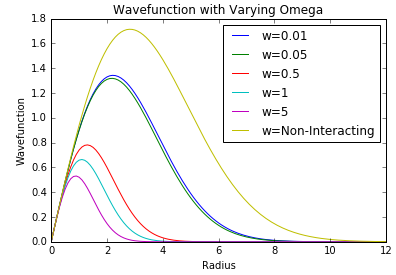
\includegraphics[width=0.525\textwidth]{C:/Users/sam61/OneDrive/Pictures/PHY480/Project2/WF_Plot.png}
	\label{}
	\caption{The wave function versus radius with varying $\omega_{r}$}
\end{figure}

Because $\omega_{r}$ is supposed to reflect the strength of the oscillator potential, it makes sense that a larger value would decrease the peak of the wave function. Should the oscillator potential be too strong, I can see the trend in this graph taking the wave function of these two electrons down to a value of zero.

I also took the interacting case, fixed $\rho_{max}$ at 5 and the matrix size at 8x8, and varied $\omega_{r}$ to see how the number of iterations were affected.

	\begin{center}
		\begin{tabular}{cc}
			\hline \hline
			$\omega_{r}$ & Iterations \\
			\hline		
			0.01 & 100  \\
			0.05  & 98 \\
			0.5 & 95 \\
			1 & 80 \\
			5 & 47 \\
			\hline
			\label{iterationsOmega}
		\end{tabular}
	\end{center}
	
Here, as well as at the previous table, a clear equation relating $\omega_{r}$ isn't obvious, but a general trend is clear. As the frequency increases in strength, the number of iterations decreases.

\section{Conclusions}
	Both the cases of one and two electrons trapped in a three-dimensional spherical potential were analyzed as eigenvalue problems and solved with Jacobi's method for diagonalizing matrices. I unexpectedly got a result that implied a degree of accuracy in the eigenvalues that rivalled the Armadillo method that is supposed to be more efficient. One case I considered as the root of this problem could be an issue where variables are stored in memory in a way such that the Armadillo eigenvalues printed off to me were actually the values on the diagonal of the final rotated matrix. 

Another, more vague suspicion I had was surrounding a quirk in the code I mentioned previously. For some reason, the algorithm would only proceed to apply rotations if the matrix was printed after each rotation (if not printed, it would stop after one transformation). It is possible this issue is tied to memory allocation and somehow affects my eigenvalues as well, but I am not sure how.

Unexpected results aside, it was shown that the number of iterations taken by Jacobi's method shrinks with the size of the matrix in the non-interacting case (and presumably in the interacting case as well). The number of iterations also shrinks with increasing values of $\omega_{r}$. Along with the increasing values of $\omega_{r}$ was a shrinking wave function, as seen in the plot, which makes sense physically given $\omega_{r}$ is a strength parameter for the oscillator potential.

	\subsection{Future Prospects}
	Solving the errors in the program noted above would be a good first step for a better analysis, as would more data points for the tables to make a more thorough argument. Also, as mentioned in the methods section, the offdiag function in the code could be optimized slightly further by not searching through the diagonal elements for the largest off-diagonal elements.

        \subsection{Acknowledgements}
        I am eternally grateful to Professor Morten Hjorth-Jensen for the C++ code examples that formed the backbone of this project, and also his unending patience and generosity when it comes to due dates. I would also like to thank John Bower for his scrutiny of my code for errors I did not end up resolving. Lastly, a special thanks to Parker Brue for aid on the wave function plots.

\begin{thebibliography}{9}
\bibitem{First}
M. Taut, Phys. Rev. A 48, 3561 (1993).
\bibitem{Second}
Hjorth-Jensen, Morten. "Computational Physics: Lecture Notes Fall 2015". Department of Physics, University of Oslo (2015).
\end{thebibliography}

\end{document}